\chapter{Background}

The purpose of this chapter is to provide the key concepts needed in detail to achieve the objectives of this project. So, in this chapter we first set out the fundamental aspects of futures trading. Next we, establish the purposes of futures contracts, then we review existing trading strategies. We then survey the most common and well-trusted evaluation strategies of trading strategies. Finally we provide an in-depth analysis on current proposed Machine Learning methods for Time Series Forecasting.

\section{Futures}
\subsection{Futures Contracts}
Futures contracts fall under a class of financial assets called `derivatives'. They are named as such because the value of a derivative is `derived' from the value of an underlying asset. A futures contract is a type of legal financial contract in which parties are obligated to buy or sell the underlying asset at a specified date in the future, at a specified price determined today, known as the \emph{forward price}. The party buying the underlying asset (at the \emph{forward price}) is said to be going \emph{long} on the contract, while the party selling the underlying asset (at the \emph{forward price}) is said to be going \emph{short} on the contract. \\ \\
The underlying asset of a future could be a commodity, such as oil, gold, and timber, stock indices such as the S\&P 500 Index, or other financial instruments. Futures contracts are used by traders to speculate about the direction of the underlying assets, and are used by businesses to \emph{hedge} or \emph{mitigate the risk} of producing or purchasing the underlying asset. \cite{jhull2017}

\section{Uses of Trading Futures}
Futures contracts have two main uses. Futures contracts can be used to speculate, or essentially realize profit based on speculation, about the underlying asset. Alternatively, futures contracts may be used to mitigate the risks associated with purchasing or producing the underlying asset. It is important to understand the motivation behind futures trading in order to reason about futures trading strategies and how they may be accelerated and optimized by machine learning techniques below.
\subsection{Trade Speculation}
The goal of a speculator in a marketplace is to make a profit by buying low and selling high. Futures allow traders to speculate on the price movement and direction of a commodity. If a speculator believes that the price of a commodity will have risen by the expiration date of a futures contract, they will take a \emph{long position}, meaning they will purchase the asset with the expectation that it will increase in value. If the price of the commodity does indeed increase beyond the original contract price, then the speculator has made a profit. This profit is realized by the speculator selling their long position at the current price of the asset. If, however, the price of the commodity decreases lower than the original contract price, the speculator has made a loss. 
\subsection{Price Risk Management via Hedging}
Financial actions and holdings have associated risks. Financial risk measures the uncertainty of rates of returns on investments. US Treasury bonds are considered to be risk-free, whereas Emerging Market equities are considered to have a high degree of risk. All trading carries some form of risk, therefore  risk management is important to protect oneself from potentially disastrous losses. \\ \\
The financial term `hedge' means `to limit'. Producers of commodities can limit the risk of producing the commodity by taking a short position in a futures contract. By entering a futures contract, producers are guaranteed to be able to sell the underlying asset, thereby hedging against any unfavourable drops in the asset's market price. Overall, hedging allows producers to transfer the risk associated with any fluctuations in the price of commodities to speculators \cite{hedge_futures}. 

\section{General Methodology For Trading}
While a trading strategy may perform well in theory, it is vitally important to evaluate the performance of trading strategies and models on real life data. Backtesting is the process of employing a strategy or model on historical data and evaluating the performance of the strategy by inspecting several important econometrics described in this section. By doing so, quantitative analysts can draw conclusions about the degree to which strategies outperform each other, identify incorrect theories that may not capture the whole picture, and improve and optimize trading strategies before they are applied to real funds.

\subsection{Equity Curve}
Equity is the sum of a trader's capital (account balance) and the profit or loss of open trades. An equity curve plots equity over time. Therefore we can observe equity curves to draw conclusions about the performance of trading strategies and models. An ideal equity curve will have a general uptrend as our goal is to generate returns. The paper Stotz, 2020 \cite{stotz_equity_curve} claims that a higher level of the equity curve is associated with higher future stock returns.

\begin{figure}[h]
    \centering
    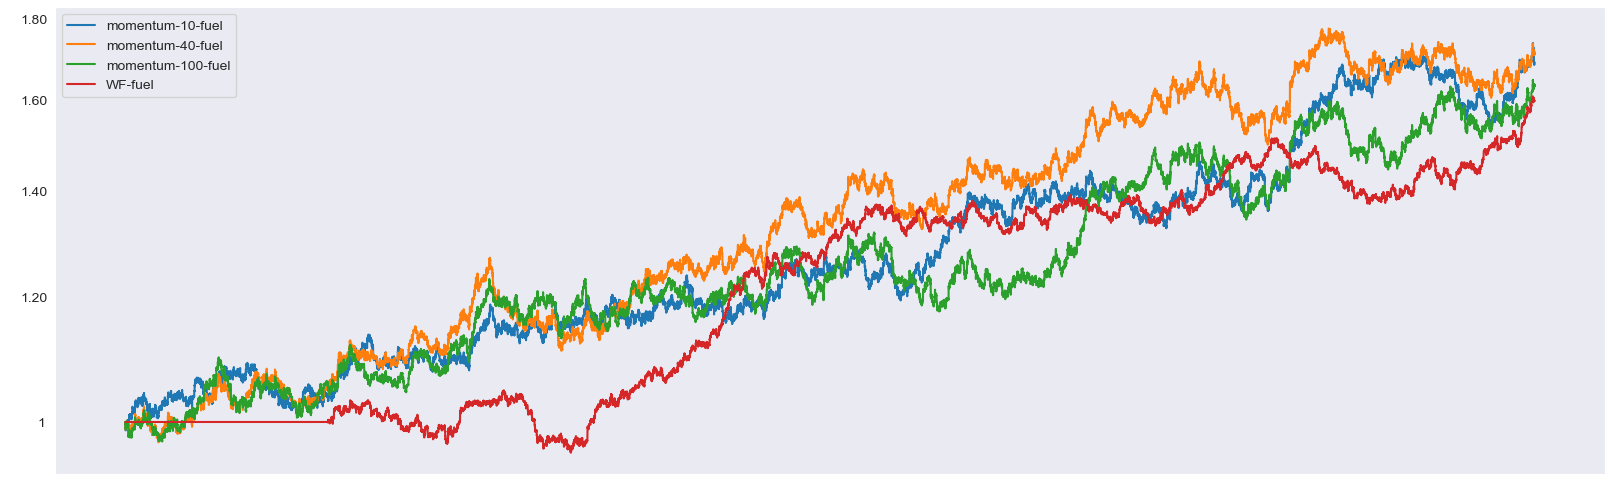
\includegraphics[scale=0.3]{background/equity_curves.png}
    \caption{Sample equity curves for comparison}
    \label{fig:my_label}
\end{figure}

\subsection{Sharpe Ratio}
The Sharpe ratio is a statistic that measures how profitable a trading strategy is, by comparing the performance of a portfolio with a risk-free asset, after adjusting returns for their risk. The Sharpe Ratio, $S_a$ is calculated using the following formula:

\begin{equation*}
S_a = \dfrac{\mathbb{E} \left[R_a - R_b \right]}{\sigma_a}
\end{equation*}

where $\mathbb{E}(x)$ is the expected value of $x$, $R_a$ is the asset return, $R_b$ is the risk free return, and $\sigma_a$ is the standard deviation of the asset excess return. The Sharpe ratio is based on mean-variance theory, and is only a valid measure of risk when the returns from an investment into an asset can be modelled by a normal distribution. Therefore, when calculated for other investments, the Sharpe ratio has a tendency to oversimplify risk. Additionally, the Sharpe ratio assumes that the return of one investment is uncorrelated with other investments within a portfolio \cite{sharpe_ratio}. 

\subsection{Max Drawdown}

The maximum drawdown (MDD) is another metric that measures the maximum drop in the value of an investment. It is calculated with the following formula:

\begin{equation*}
    MDD(T) = \dfrac{\text{Trough Value} - \text{Peak Value}}{\text{Peak Value}}
\end{equation*}
where $MDD(T)$ is the maximum drawdown at time $T$, the `Peak Value' is the peak value of the investment before the largest drop in its value at time $T$, and `Trough Value' is the lowest value of the investment before a new peak is attained. \\ \\
As cited in (Petroni and Rotundo, 2008) \cite{PETRONI20083942}, MDD is one of the most widely quoted measurements of risk, as it is an indicator of downside risk. The authors mention that decreasing trends can force investors to abandon a market. Funds with relatively low MDDs have an out-of-sample alpha of 2.40\% as claimed in Riley and Yan, 2022 \cite{max_drawdown}. Figure 2.2 shows a typical MDD plot for various trading strategies.

\begin{figure}[h]
    \centering
    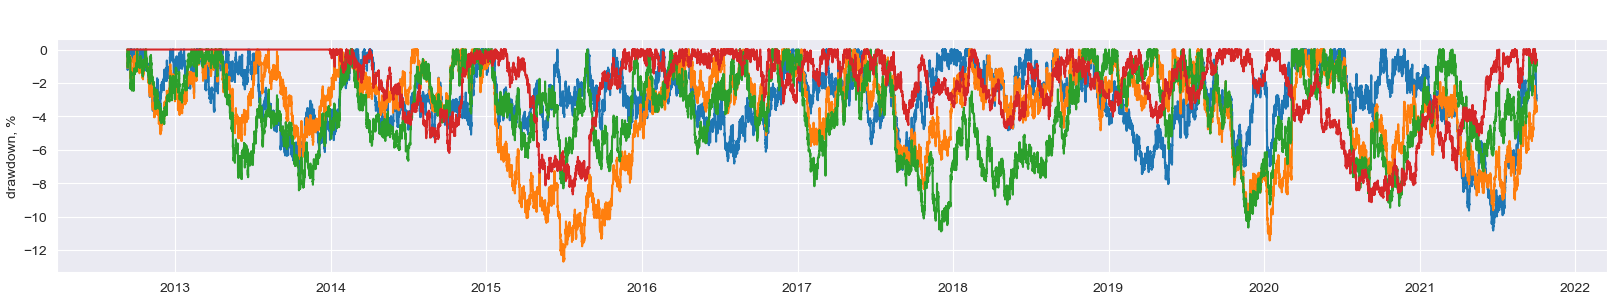
\includegraphics[scale=0.25]{background/drawdown.png}
    \caption{Sample Max Drawdown Plot Comparison for Various Trading Strategies}
    \label{fig:my_label}
\end{figure}

\subsection{Momentum}
Momentum-based trading strategies are widely used and well-known amongst practitioners. Momentum is a key observed behaviour of asset prices, where if the price of an asset rises, it will continue to rise. Similarly, if the price of an asset falls, it will continue to fall. One example of a momentum-based statistical model is ARIMA (Auto-regressive Integrated Moving Average). Two major distinct subsets of momentum-based strategies are time-series momentum and cross-sectional momentum. \\ \\
Both strategies rely on momentum; both strategies include the selection of investments based on their past performance. Cross-sectional momentum strategies involve the observation of relative past performance of securities. The key idea is that securities that have managed to outperform peers in the past are likely to continue to outperform. Such securities are typically labeled `winners'. On the other hand, time-series momentum, proposed by Moskowitz et al. (2012) \cite{moskowitz2012time}, observes the past performance of an individual security, otherwise known as the absolute performance. The main idea is that securities that have managed to yield a return over a certain threshold are likely to continue to perform well. \cite{bird2017time}

\subsection{Volatility Targeting and Scaling}
Targeting certain levels of risk when designing a trading system is important to avoid overconfidence and cut losses \cite{carver2015systematic}. The theory behind volatility-managed portfolios is described in recent work by Moreira and Muir (2016) \cite{moreira_muir}. The authors mention that portfolios that are scaled down during periods of high volatility generate large alphas (excess returns) and increase Sharpe ratios. In the 2018 paper `The Impact of Volatility Targeting' \cite{vol_target} the authors investigate the impact of leveraging a portfolio when market volatility is low, and scaling down a portfolio when the market experiences heightened levels of uncertainty.

\subsection{Backtesting Methodology}
Backtesting applies trading strategies to historical data, which allows one to observe the performance of a strategy, identify theoretical gaps in implementations, and compare strategies against one another. Backtesting is used under the assumption that if a trading strategy performed well in the past, there is a good chance of the strategy performing in the future, and similarly for trading strategies that do not perform desirable backtesting results. \cite{backtesting_impl}.

\subsection{Walkforward Methodology}
When machine learning algorithms attempt to model the relationship between time and financial data, there are certain hyperparameters specific to each algorithm that influence the performance of the model, such as decreasing the risk of overfitting. While classical cross-validation methods for classification tasks are not applicable to time-series data, Walk-Forwards Optimization (WFO) is a prominent, widely-used alternative. WFO preserves the temporal ordering of times-series data by applying a `sliding window' over data. Each window has an 'in-sample' period on which data is trained.  Then the hyperparameters of the model are tuned by observing the accuracy of the model on the remaining data in the window, called the `held-out' or `out-of-sample' period data \cite{bilkon_ml}. 



% IF THERE IS TIME, WRITE PARAGRAPHS ABOUT VOLATILITY NORMALISATION AND THE BACKTESTING FRAMEWORK ARCHITECTURE
% \subsection{Volatility Normalisation}
% \textbf{TO COMPLETE}

% \subsection{Backtesting Framework Architecture}
% \textbf{TO COMPLETE}
\section{Time Series Forecasting}
Time series forecasting is a fundamental technique which utilizes historical data to predict future values of a certain quantity, and is thus integral for constructing machine learning algorithms that form futures trading strategies. Financial time series forecasting, however, is seen to be one of the most challenging applications of modern time series forecasting, as financial time series are inherently noisy, non-stationary and deterministically chaotic. The chaotic and noisy nature of financial time series is a result of the unavailability of complete information \cite{svm-fts} about the influence of past market behaviour on future prices, as well as many non-linear factors such as GDP growth, economic policies etc. Overall, time-series forecasting can reveal novel insights about the relationships between variables in historical time series data.

\subsection{Alpha Generation}

In finance terms, alpha generation is the process of generating absolute returns, known as `alpha'. Alpha generation is a complex process based on computer algorithms and programs that are capable of making quick predictions based on past performances involving large datasets. Alpha indicates the excess return of an investment relative to the return of a benchmark index such as the S\&P 500. Hedge funds employ complex strategies to generate alpha \cite{alpha_hf}. Generating alpha is difficult to sustain over the long term; many actively managed mutual funds fail to outperform their benchmarks over the long term. For example, 99 large-cap funds outperformed the S\&P 500 index in the 3 years prior to September 30th 2016, however none of the funds had been able to outperform the index by the end of September 2019 \cite{alpha_ch}. 

\section{Machine Learning Methods for Time Series Forecasting}
Machine learning algorithms for regression (prediction) tasks lend themselves to the problem of time-series forecasting as models can synthesize large datasets, identify patterns optimally, and produce trading strategies without the emotions and bias of human traders. 

\subsection{Linear Regression}
Given a set of explanatory (input) variables, $\{x_1^{(i)}, x_1^{(i)},  ..., x_1^{(i)}\}_{i=1}^N$ and a forecast (output) variable $\{y^{(i)}\}_{i=1}^N$, a linear regression model assumes that the relationship between the descriptor variables and the forecast variable is linear. Therefore a linear regression model takes the form:

\begin{equation*}
    y^{(i)} = \beta_0 + \beta_1x_1^{(i)} + \beta_2x_2^{(i)} ... + \beta_px_p^{(i)} + \varepsilon^{(i)}
\end{equation*}
where $\beta_0, ... , \beta_p$ are the parameters/weights of the model to be determined by fitting the model to sample data, and $\varepsilon^{(i)}$ is a Gaussian noise term. 
\subsection{Random Forest}
Random forest is an ensemble of decision tree algorithms that has been applied to regression tasks for time-series forecasting. The random forest algorithm involves generating many decision trees that are trained on `bootstrap samples' (introduced in Efron and Tibshirani, 1993) \cite{bootstrap}, which involve drawing samples without replacement from a training dataset. Each decision tree outputs a predicted value given a sample of training data. Finally, the output prediction of random forest is the average prediction across the decision trees. An application of random forest in time-series forecasting is described in Mei et al, 2014. The paper claims that random forest time-series predictions  produced a Mean Absolute Percentage Error (MAPE) of 12.03\%, in comparison to an Autoregressive-moving-average (ARMA) statistical model which achieved an MAPE of 13.65\%. \cite{mei2014random}.

\section{Deep Learning For Time-Series Forecasting}
The acceleration of deep learning models in the past few decades has given rise to a number of high performance, vastly adaptable deep learning models and architectures that can be employed for time-series forecasting. As deep learning is mainly concerned with graph architectures that use multiple inputs and outputs, deep learning neural networks are capable of capturing additional information that may accompany time-series data, for example `boom and bust' cycles or seasonal trends. Therefore deep learning is extremely valuable in time-series forecasting.

\subsection{Artificial Neural Networks}
Artificial neural networks consist of a network of neurons arranged in layers, where each neuron transmits signals to further neurons. Neural networks have been adapted to perform time-series prediction, as described in Frank et al. (2001) \cite{frank2001time}. Figure 2.3 shows a typical Artificial neural network architecture.

\begin{figure}[!h]
    \centering
    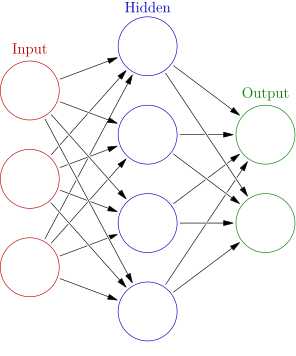
\includegraphics[scale=0.4]{Colored_neural_network.png}
    \caption{Artificial Neural Network Architecture}
    \label{fig:my_label}
\end{figure}

\break
\subsection{LSTMs}
\label{lstms+transforms}
 As opposed to basic neural networks, LSTMs, which are a kind of Recurrent Neural Networks (RNN), consist of connections between neurons that form cycles; in other words, the feedback connections allow for the output of some neurons to be used as inputs to those neurons. Therefore RNNs have some internal representation of `memory'. RNNs use current input and what it has learned on previous data to complete its task. RNNs were developed to work on tasks involving time-series data, and thus RNNs are typically used in combination with time-series data preparation methods such as \emph{rolling sliding window}. \\ \\
A significant development on RNNs are LSTM neural networks, which were first introduced by Hochreiter and Schmidhuber, 1997 (\cite{hochreiter1997long}). The internal architecture of LSTMs consists of `memory cells' that can remember the historical context of data. As mentioned in Lazzeri, 2021, due to the `memory cell' architecture of LSTMs, these neural networks can learn about dependencies between inputs in a temporal order and an output \cite{lazzeri2020machine}. Figure 2.4 shows a typical LSTM architecture.

\begin{figure}[h]
    \centering
    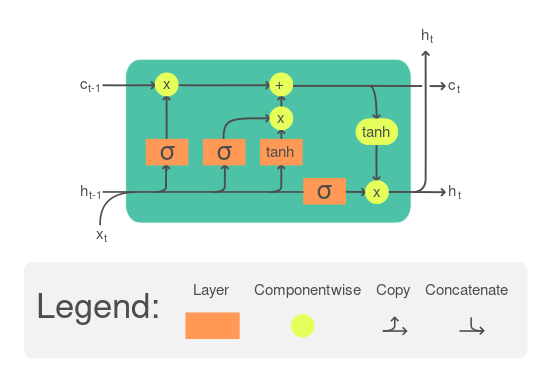
\includegraphics[scale=0.5]{background/LSTM_Cell.png}
    \caption{Typical LSTM Architecture}
    \label{fig:my_label}
\end{figure}

\subsection{Ensemble Methods}
Ensemble methods aim to improve the overall performance of machine learning algorithms by combining several models instead of relying one one method. Overall predictions are usually decided on by taking a `weighted vote` of the predictions of the individual models as described in Dietterich, 2000 \cite{dietterich2000ensemble}. The paper describes several strategies to achieve performant ensemble models such as Bayesian Voting \cite{dietterich2000ensemble}, Bagging \cite{bootstrap},  omitting various input features from the individual models, and a technique described by Dietterich and Bakiri (1995) as `error-correcting output coding' \cite{dietterich1994solving}. \\ \\
In Oliveira and Torgo, 2014 \cite{acml2014}, ensemble methods and techniques are reviewed in the context of time-series forecasting. 
 
\subsection{Meta-Labelling}
Meta-labelling is introduced in Lopez de Prado, 2018. Meta-labelling includes using a binary prediction from one classifier, then using the probability that the prediction was made to make further decisions about the extent to which the prediction should be accepted. Lopez de Prado mentions that meta-labelling can help to drop false positive predictions, thereby increasing the F1 score of a model \cite{marcos}.

\subsection{L1 and L2 Regularization}
\label{l1l2}
L1 \cite{tibshirani1996regression} and L2 regularization \cite{hoerl1970ridge} are methods to shrink the influence of features that are deemed less important in machine learning models. By restricting the number of features influencing the predictions of models, these models are discouraged from becoming too complex and overfitting on data.

\subsection{Challenges}
\label{challenges}
Machine learning and deep learning models are prone to underfitting or overfitting data. During underfitting, models will perform poorly on training datasets as well as test datasets, whereas during overfitting, models will typically perform badly on test datasets, thus displaying that the model does not generalize well to unseen data. Therefore it is important that datasets provide a representative sample of the population on which the models will predict. Additionally, ML/DL models are typically not designed to work on sequential data, therefore models must be adapted to suit time-series data, and this data may need to undergo some preparation before models can work effectively on it.

\subsection{Deep Learning Framework}
Time Series AI (TSAI), a deep learning framework with libraries designed to work on time series data and sequences, is built using \texttt{PyTorch} and \texttt{fastai}. TSAI includes implementations of several state-of-the-art deep learning models that can be adapted for time series forecasting, including LSTMs \hyperref[lstms+transforms]{(Section 2.5.5)}, Multilayer Perceptron and Time Series Transformers (Zerveas et al, 2021) \cite{10.1145/3447548.3467401}. Functionalities of TSAI includes data preparation methods (e.g sliding window as described in \hyperref[wfo]{Section 2.3.3}), data augmentation and prediction analysis (including visualization), as outlined in TSAI documentation. \cite{tsai}
\subsection{Project Data (Time Series)}
All data in this project will be primarily sourced from \href{https://github.com/apache/parquet-format}{Apache Parquets}, which is an open source column-based data format,  containing prices and return data for selected futures contracts for major commodities: emerging markets, agricultural futures (e.g cocoa, orange juice), equity indices (e.g E-mini S\&P 500), fuel (e.g Brent Last Day Financial) and metals (e.g gold). The parquet files contain time series data from 2012 to 2021 on futures contracts. We will use this data to fit and test our ML models, backtest the strategies produced, and to compare different strategies. 

\begin{figure}[h]
    \centering
    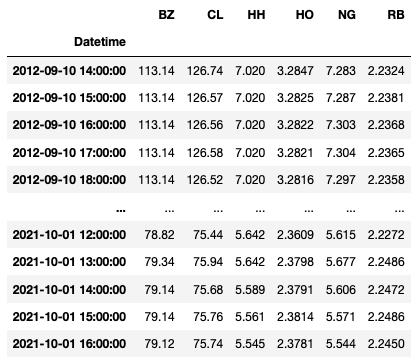
\includegraphics[scale=0.5]{background/Screenshot 2023-01-25 at 00.08.54.png}
    \caption{Sample data file}
    \label{fig:my_label}
\end{figure}
% DATA
% 1. What is the source of data?
% 2. What is the data?
% 3. What are you going to do with the data? And how are you going to do?

% Ask teacher, I'm going to include these things about the data, is there anything else I could include?
% 30 min to write TSAI, 30 min to write data